\documentclass[tikz,border=6pt]{standalone}
\usetikzlibrary{arrows.meta,positioning,fit}
\begin{document}
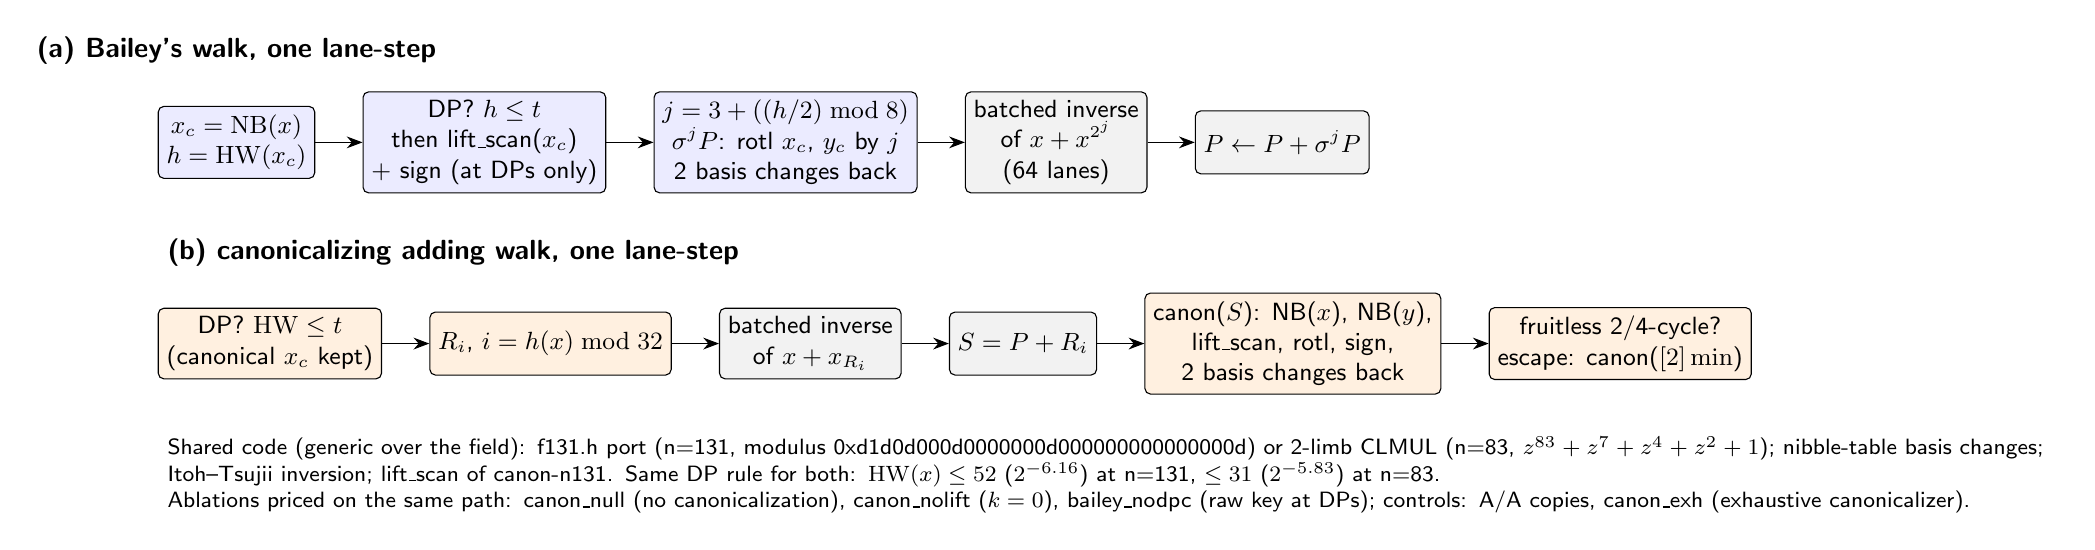
\begin{tikzpicture}[font=\sffamily\small, node distance=4mm and 6mm,
  box/.style={draw, rounded corners=2pt, align=center, minimum height=8mm, inner sep=3pt},
  a/.style={box, fill=blue!8}, b/.style={box, fill=orange!12}, s/.style={box, fill=gray!10},
  ar/.style={-{Stealth[length=2mm]}}]
\node[font=\sffamily\bfseries] (ta) {(a) Bailey's walk, one lane-step};
\node[a, below=of ta] (a1) {$x_c=\mathrm{NB}(x)$\\ $h=\mathrm{HW}(x_c)$};
\node[a, right=of a1] (a2) {DP? $h\le t$\\ then lift\_scan($x_c$)\\ + sign (at DPs only)};
\node[a, right=of a2] (a3) {$j=3+((h/2)\bmod 8)$\\ $\sigma^j P$: rotl $x_c$, $y_c$ by $j$\\ 2 basis changes back};
\node[s, right=of a3] (a4) {batched inverse\\ of $x+x^{2^j}$\\ (64 lanes)};
\node[s, right=of a4] (a5) {$P\leftarrow P+\sigma^j P$};
\draw[ar] (a1)--(a2); \draw[ar] (a2)--(a3); \draw[ar] (a3)--(a4); \draw[ar] (a4)--(a5);
\node[font=\sffamily\bfseries, below=14mm of a1.west, anchor=west] (tb) {(b) canonicalizing adding walk, one lane-step};
\node[b, below=of tb.south west, anchor=north west] (b1) {DP? $\mathrm{HW}\le t$\\ (canonical $x_c$ kept)};
\node[b, right=of b1] (b2) {$R_i$, $i=h(x)\bmod 32$};
\node[s, right=of b2] (b3) {batched inverse\\ of $x+x_{R_i}$};
\node[s, right=of b3] (b4) {$S=P+R_i$};
\node[b, right=of b4] (b5) {canon($S$): NB($x$), NB($y$),\\ lift\_scan, rotl, sign,\\ 2 basis changes back};
\node[b, right=of b5] (b6) {fruitless 2/4-cycle?\\ escape: canon($[2]\min$)};
\draw[ar] (b1)--(b2); \draw[ar] (b2)--(b3); \draw[ar] (b3)--(b4); \draw[ar] (b4)--(b5); \draw[ar] (b5)--(b6);
\node[align=left, below=6mm of b1.south west, anchor=north west, text width=24cm, font=\sffamily\footnotesize] (n)
 {Shared code (generic over the field): f131.h port (n=131, modulus 0xd1d0d000d0000000d000000000000000d) or 2-limb CLMUL (n=83, $z^{83}+z^7+z^4+z^2+1$);
  nibble-table basis changes; Itoh--Tsujii inversion; lift\_scan of canon-n131. Same DP rule for both: $\mathrm{HW}(x)\le 52$ ($2^{-6.16}$) at n=131, $\le 31$ ($2^{-5.83}$) at n=83.\\
  Ablations priced on the same path: canon\_null (no canonicalization), canon\_nolift ($k=0$), bailey\_nodpc (raw key at DPs); controls: A/A copies, canon\_exh (exhaustive canonicalizer).};
\end{tikzpicture}
\end{document}
